\chapter{Préambule}
\epigraph{Le chemin est long du projet à la chose.}{Molière}

\section{Comment compiler ce document ?}

Un document \LaTeX peut se compiler au travers d'un IDE (TexSutdio, TeXMaker par exemple).
Le répertoire de ce document contient également un Makefile qui permet de compiler simplement en ligne de commande. 
La fabrication du glossaire et de l'index est prise en charge par ce Makefile.
Pour l'utiliser, il suffit d'ouvrir un terminal, de se placer dans le répertoire du document puis d'invoquer la commande \texttt{make}. 


Voici les différentes cibles disponibles pour ce Makefile :
\begin{verbatim}
make                - contruit le document
make all            - contruit le document
make index          - contruit l'index
make glossaire      - contruit le glossaire
make bib            - contruit la bibliographie
make pdf            - contruit le document PDF
make clean          - supprime les fichiers LaTeX intermédiaires
make clean-all      - supprime tous les fichiers générés par la compilation
make help           - cette information
\end{verbatim}


\section{Références internes}

Les références internes sont des renvois vers des figures, des tableaux ou des sections du rapport.
\LaTeX introduit un mécanisme simple pour établir ce genre de référence, via les commandes \texttt{\textbackslash label} et \texttt{\textbackslash ref}. 
La première sert à définir une ancre dans le document, la seconde à la citer.
Voici par exemple une référence interne vers la section intitulée \textit{Approche Top-Down} (cf. section  \ref{sec:top-down}). Ce renvoi est le résultat de la commande \texttt{\textbackslash ref\{sec:top-down\}}. Si vous vous rendez dans le corps de cette section, vous y trouverez le label en question \texttt{\textbackslash label\{sec:top-down\}}. 

\subsection{Tableaux et figures}
Les figures  et les tableaux  sont référencés de la même la manière (cf. figure \ref{fig:gomboc} et tableau \ref{tab:exemple}). \index{Table} \index{Figure}

\begin{table}[h]
\centering
\begin{tabular}{lll}
\toprule
\textbf{Algorithmes} & \textbf{Performance (s)} & \textbf{Gain (dB)}\\
\midrule
Algorithme 1 & 0.0003262 & 0.562 \\
Algorithme 2 & 0.0015681 & 0.910 \\
Algorithme 3 & 0.0009271 & 0.296 \\
\bottomrule
\end{tabular}
\caption{\label{tab:exemple}Performances et gains des algorithmes envisagés.}
\end{table}

\begin{figure}[h]
\centering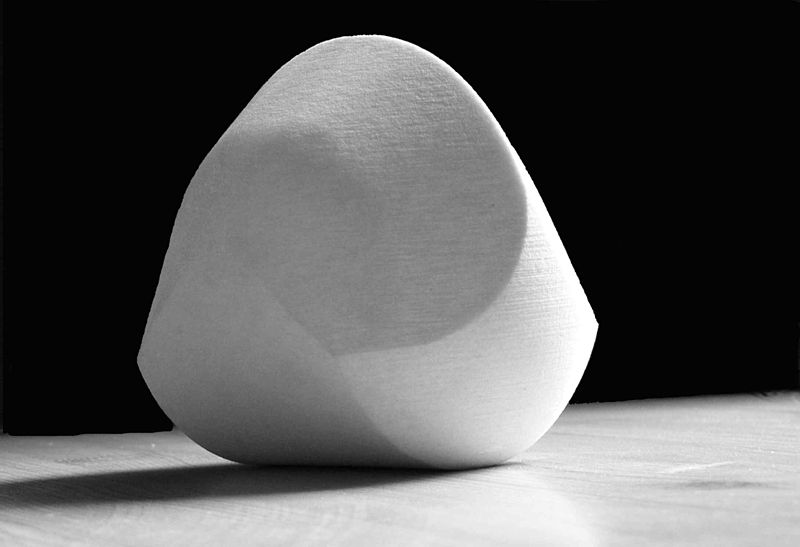
\includegraphics[scale=0.15]{Gomboc.jpg}
\caption{\label{fig:gomboc}Gömböc : un objet homogène tridimensionnel mono-monostatique. (source : Wikipedia)}
\end{figure}



\subsection{Codes}
Si vous souhaitez insérer du code dans votre rapport, invoquez les commandes : \\
 \texttt{\textbackslash lstset\{language=python\}}\\
 \texttt{\textbackslash lstinputlisting[caption=\{Titre du listing\}, label=\{lst:code\}]\{./code/code.py\}}


La première commande sélectionne le langage, pour que les mots clés de celui-ci soit correctement détectés et mis en valeur. 
La seconde commande permet d'insérer le code contenu dans le fichier code.py qui se trouve dans le sous-répertoire code.
Pour faire référence au code, il suffit de sélectionner le label du listing \ref{lst:prime},  comme pour les figures et les tableaux.

\lstset{language=python}
\lstinputlisting[caption={Titre du listing}, label={lst:prime}]{./code/primegen.py}


\subsection{Index et glossaire}

Pour insérer des entrées dans l'index, il suffit de déclarer des mots via la commande \texttt{\textbackslash index\{Fabrication d'un index\}} comme suit\footnote{Allez donc voir l'index \ref{sec:index} à la fin du document  !}. \index{Fabrication d'un index}

Pour utiliser le glossaire, il faut définir les termes dans le fichier \texttt{glossaire.tex} en utilisant la commande \texttt{\textbackslash newacronym\{label\}\{abbréviation\}\{Signification\}}. 
Puis,  \texttt{\textbackslash gls\{label\}} permet de les utiliser dans le document. 


Par exemple, les UVs 3.4 et 4.4 sont une initiation à l'\gls{IS}. 
Un concept de gestion de projet souvent mal connu est le \gls{WBS}.


\section{Références bibliographiques}

Les références bibliographiques sont des documents numériques, des livres, des articles, des images ou des vidéos qui ne sont pas présents dans le rapport. 
\LaTeX propose un mécanisme simple de citation.
Pour plus de détails, vous pouvez consulter les références suivantes \cite{maguis2010redigez,desgraupes2003latex,bitouze2010latex} qui sont présentent à la médiathèque de l'ENSTA Bretagne, ou celle-ci directement sur le web \cite{openclassroomLaTeX}.  

Pour citer des documents, il suffit d'appeler la commande \texttt{\textbackslash cite\{key\}} en choisissant la clé qui identifie le document, comme suit : \cite{lamport1985i1}. 
Cette clé de citation est celle qui référence l'ouvrage dans le fichier de bibliographie intitulé   \texttt{bibliographie.bib}.
Ce fichier d'exemple contient tous les types de documents dont vous aurez besoin : livre, article de journal, références web,  rapport\dots 
Une fois insérée et compilée, la citation devient un lien dans le fichier pdf, redirigeant ainsi directement vers le détail de l'ouvrage cité dans la bibliographie située à la fin du document.
 
